\begin{tabular}{M{6.5cm}M{11cm}}
	\textbf{LỚP CÔ THẢO - THẦY SANG}& \textbf{ĐỀ ÔN TẬP KIỂM TRA GIỮA HỌC KÌ 1}\\
	\textbf{MÃ ĐỀ: 001}& \textbf{Bài thi môn: VẬT LÝ 10}\\
	\textit{(Đề thi có 06 trang)}& \textit{Thời gian làm bài: 50 phút, không kể thời gian phát đề}
	
	\noindent\rule{4cm}{0.8pt} \\
\end{tabular}
\setcounter{section}{0}
\section{Câu trắc nghiệm nhiều phương án lựa chọn}
\textit{Thí sinh trả lời từ câu 1 đến câu 18. Mỗi câu hỏi thí sinh chọn một phương án}
\setcounter{ex}{0}
\Opensolutionfile{ans}[ans/G10-4-TN]
% ===================================================================
\begin{ex}
	Đối tượng nghiên cứu của vật lí là gì?
	\choice
	{Các dạng vận động và tương tác của vật chất}
	{Quy luật tương tác của các dạng năng lượng}
	{\True Các dạng vận động của vật chất và năng lượng}
	{Quy luật vận động, phát triển của sự vật - hiện tượng}
	\loigiai{}
\end{ex}
% ===================================================================
\begin{ex}
	Chọn phát biểu \textbf{đúng}.
	\choice
	{Vận tốc tức thời cho ta biết chiều chuyển động của vật nên luôn có giá trị dương}
	{Vector độ dịch chuyển thay đổi phương liên tục khi vật chuyển động thẳng}
	{\True Khi vật chuyển động thẳng không đổi chiều, độ lớn của vector độ dịch chuyển bằng quãng đường vật đi được}
	{Vector độ dịch chuyển có độ lớn luôn bằng quãng đường đi được của chất điểm}
	\loigiai{}
\end{ex}
% ===================================================================
\begin{ex}
	Tốc độ là đại lượng đặc trưng cho
	\choice
	{\True tính chất nhanh hay chậm của chuyển động}
	{sự thay đổi hướng của chuyển động}
	{khả năng duy trì chuyển động của vật}
	{sự thay đổi vị trí của vật trong không gian}
	\loigiai{}
\end{ex}
% ===================================================================
\begin{ex}
	Chuyển động thẳng chậm dần đều là chuyển động có
	\choice
	{tốc độ giảm đều, gia tốc giảm đều}
	{vận tốc không đổi, gia tốc giảm đều}
	{\True tốc độ giảm đều, gia tốc không đổi}
	{vận tốc không đổi, gia tốc không đổi}
	\loigiai{}
\end{ex}
% ===================================================================
\begin{ex}
	Trong các hoạt động dưới đây, hoạt động nào tuân thủ nguyên tắc an toàn khi làm việc với các nguồn phóng xạ?
	\choice
	{Ăn uống, trang điểm trong phòng làm việc có chứa chất phóng xạ}
	{\True Sử dụng phương tiện phòng hộ cá nhân như quần áo phòng hộ, mũ, găng tay, áo chì, \dots}
	{Đổ rác thải phóng xạ tại các khu tập trung rác thải sinh hoạt}
	{Dùng hộp chứa bằng vật liệu thuỷ tinh để đựng chất phóng xạ}
	
	\loigiai{}
\end{ex}
% ===================================================================
\begin{ex}
	Chọn đáp án có từ/cụm từ thích hợp để hoàn thành các câu sau:
	\begin{itemize}
		\item[-] Các số hạng trong phép cộng (hoặc trừ) phải có cùng (1) \dots và nên chuyển về cùng (2) \dots.
		\item[-] (3) \dots của một biểu thức vật lí phải có cùng thứ nguyên.
	\end{itemize}
	\choice
	{(1) đơn vị; (2) thứ nguyên; (3)  Đại lượng}
	{(1) thứ nguyên; (2) đại lượng; (3) Hai vế}
	{(1) đơn vị; (2) đại lượng; (3) Hai vế}
	{\True (1) thứ nguyên; (2) đơn vị; (3) Hai vế}
	\loigiai{}
\end{ex}
% ===================================================================
\begin{ex}
	Trong các phép đo dưới đây, đâu là phép đo trực tiếp?
	\begin{enumerate}[label=(\arabic*)]
		\item Dùng thước đo chiều cao.
		\item Dùng cân đo cân nặng.
		\item Dùng cân và ca đong đo khối lượng riêng của nước.
		\item Dùng đồng hồ và cột cây số đo tốc độ của người lái xe.
	\end{enumerate}
	\choice
	{\True (1), (2)}
	{(1), (2), (4)}
	{(2), (3), (4)}
	{(2), (4)}
	\loigiai{}
\end{ex}
% ===================================================================
\begin{ex}
	Đâu là cách viết kết quả đo \textbf{đúng}?
	\choice
	{$A=\overline{A}+\Delta A$}
	{$A=\overline{A}-\Delta A$}
	{\True $A=\overline{A}\pm\Delta A$}
	{$A=\overline{A}:\Delta A$}
	\loigiai{}
\end{ex}

% ===================================================================
\begin{ex}
	Một vật chuyển động thẳng có đồ thị vận tốc theo thời gian như hình vẽ. Giai đoạn vật chuyển động thẳng nhanh dần đều là
	\begin{center}
		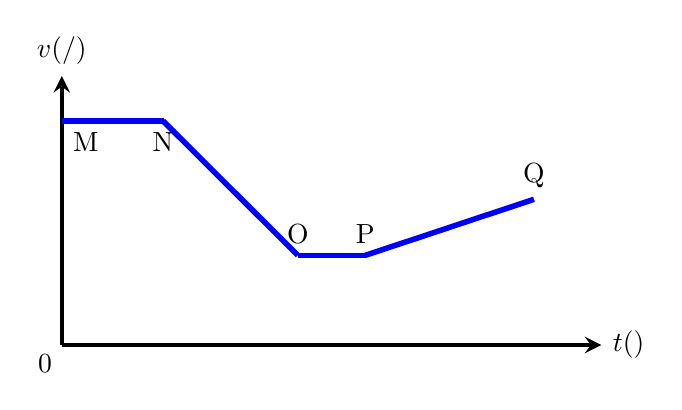
\begin{tikzpicture}  
			\begin{axis}[  ultra thick,yscale=0.6,
				xmin=0,  
				xmax=16,  
				ymin=0,  
				ymax=6, 
				samples=300,
				yticklabels=\empty,
				xticklabels=\empty,
				xtick=\empty,
				ytick=\empty,
				axis lines=center, 
				xlabel=$\xsi{t}{\left(\si{\second}\right)}$, 		ylabel=$\xsi{v}{\left(\si{\meter/\second}\right)}$,
				every axis y label/.style={at=(current axis.above origin),anchor=south},  
				every axis x label/.style={at=(current axis.right of origin),anchor=west},  ]
				\coordinate (M) at (axis cs: 0,5);
				\coordinate (N) at (axis cs: 3,5);
				\coordinate (OO) at (axis cs: 7,2);
				\coordinate (P) at (axis cs: 9,2);
				\coordinate (Q) at (axis cs: 14,3.25);
				\addplot [line width=2pt, blue, smooth, domain=0:3] {5}; 
				\addplot [line width=2pt, blue, smooth, domain=3:7] {5-0.75*(x-3)}; 
				\addplot [line width=2pt, blue, smooth, domain=7:9] {2}; 
				\addplot [line width=2pt, blue, smooth, domain=9:14] {2+0.25*(x-9)};
				\coordinate (O) at (axis cs: 0,0);
				\node[below right] at (M) {M};
				\node[below] at (N) {N};
				\node[above] at (OO) {O};
				\node[above] at (P) {P};
				\node[above] at (Q) {Q};
			\end{axis}  
			\node[below left] at (O) {0};
		\end{tikzpicture}
	\end{center}
	\choice
	{MN}
	{NO}
	{OP}
	{\True PQ}
	\loigiai{}
\end{ex}
% ===================================================================
\begin{ex}
	Bạn Bình đi học từ nhà đến trường theo lộ trình ABC như hình vẽ. Biết bạn Bình đi đoạn đường $\mathrm{AB}=\SI{400}{\meter}$ hết 6 phút, đoạn đường $\mathrm{BC}=\SI{300}{\meter}$ hết 4 phút. Vận tốc trung bình của bạn Bình khi đi từ nhà đến trường là
	\begin{center}
		\includegraphics[width=0.4\linewidth]{../figs/D10-1-3}
	\end{center}
	\choice
	{\True $\SI{0.833}{\meter/\second}$}
	{$\SI{2.916}{\meter/\second}$}
	{$\SI{1.167}{\meter/\second}$}
	{$\SI{3.512}{\meter/\second}$}
	\loigiai{
	$$v=\dfrac{\mathrm{AC}}{t_{\mathrm{AB}}+t_{\mathrm{BC}}}\approx\SI{0.833}{\meter/\second}.$$
	}
\end{ex}
% ===================================================================
\begin{ex}
	Giờ Phối hợp Quốc tế (UTC) là tiêu chuẩn thời gian được sử dụng rộng rãi trên thế giới. So với 0 giờ Quốc Tế, Việt Nam ở múi giờ thứ 7 (UTC +7) và Nhật Bản ở múi giờ thứ 9 (UTC +9). Ngày 10/02/2024, máy bay VN300, thuộc hãng hàng không Vietnam Airlines, khởi hành từ Thành phố Hồ Chí Minh lúc 0 giờ 20 phút và đến Thành phố Tokyo lúc 7 giờ 45 phút, theo giờ địa phương. Thời gian di chuyển của máy bay này là
	\choice
	{5 giờ 25 phút}
	{\True 9 giờ 25 phút}
	{7 giờ 25 phút}
	{8 giờ 05 phút}
	\loigiai{
	}
\end{ex}

% ===================================================================
\begin{ex}
	Biểu thức nào sau đây đang mô tả vận tốc của vật chuyển động thẳng chậm dần đều?
	\choice
	{\True $v=-20+5t\ \left(\si{\meter/\second}; \si{\second}\right)$}
	{$v=10+5t\ \left(\si{\meter/\second}; \si{\second}\right)$}
	{$v=5t\ \left(\si{\meter/\second}; \si{\second}\right)$}
	{$v=-20-5t\ \left(\si{\meter/\second}; \si{\second}\right)$}
	\loigiai{}
\end{ex}
% ===================================================================
\begin{ex}
	Một vật chuyển động thẳng nhanh dần đều với tốc độ đầu là $\SI{6}{\meter/\second}$ và độ lớn gia tốc là $\SI{2}{\meter/\second^2}$. Chọn thời điểm ban đầu là lúc vật ở gốc tọa độ và chiều dương ngược chiều chuyển động thì phương trình chuyển động của vật có dạng
	\choice
	{$x=6t-t^2\ \left(\si{\meter}; \si{\second}\right)$}
	{$x=6t-2t^2\ \left(\si{\meter}; \si{\second}\right)$}
	{\True $x=-6t-t^2\ \left(\si{\meter}; \si{\second}\right)$}
	{$x=-6t-2t^2\ \left(\si{\meter}; \si{\second}\right)$}
	\loigiai{}
\end{ex}
% ===================================================================
\begin{ex}
	Một xe đi nửa đoạn đường đầu tiên với tốc độ trung bình
	 $v_1=\SI{12}{\kilo\meter/\hour}$ và nửa đoạn đường	sau với tốc độ trung bình $v_2=\SI{20}{\kilo\meter/\hour}$. Tốc độ trung bình của xe trên cả đoạn đường là
	\choice
	{$\SI{30}{\kilo\meter/\hour}$}
	{\True $\SI{15}{\kilo\meter/\hour}$}
	{$\SI{16}{\kilo\meter/\hour}$}
	{$\SI{32}{\kilo\meter/\hour}$}
	\loigiai{
	$$v_{\text{tb}}=\dfrac{2s}{\dfrac{s}{v_1}+\dfrac{s}{v_2}}=\dfrac{2}{\dfrac{1}{v_1}+\dfrac{1}{v_2}}=\SI{15}{\kilo\meter/\hour}.$$
	}
\end{ex}
% ===================================================================
\begin{ex}
	Một ô tô đang chạy với vận tốc $\SI{72}{\kilo\meter/\hour}$ trên một đoạn đường thắng thì người lái xe hãm phanh cho ô tô chạy chậm dần. Sau $\SI{40}{\second}$, ô tô dừng lại. Gia tốc của ô tô là
	\choice
	{$a=\SI{-0.2}{\meter/\second^2}$}
	{\True $a=\SI{-0.5}{\meter/\second^2}$}
	{$a=\SI{0.2}{\meter/\second^2}$}
	{$a=\SI{-1}{\meter/\second^2}$}
	\loigiai{
	$$a=\dfrac{v-v_0}{\Delta t}=\dfrac{0-20}{40}=\SI{-0.5}{\meter/\second^2}.$$
	}
\end{ex}

% ===================================================================
\begin{ex}
	Một xe máy đang chạy với tốc độ $\SI{36}{\kilo\meter/\hour}$ bỗng người lái xe thấy có một cái hố trước mặt, cách xe $\SI{20}{\meter}$. Người ấy phanh gấp và xe đến ngay trước miệng hố thì dừng lại. Gia tốc của xe máy có độ lớn là 
	\choice
	{$\SI{5.09}{\meter/\second^2}$}
	{$\SI{4.1}{\meter/\second^2}$}
	{\True $\SI{2.5}{\meter/\second^2}$}
	{$\SI{32.4}{\meter/\second^2}$}
	\loigiai{}
\end{ex}

% ===================================================================
\begin{ex}
	Một vật chuyển động trên đường thẳng có phương trình vận tốc - thời gian $v=-5+5t\ \left(\si{\meter/\second};\si{\second}\right)$. Tại thời điểm $t=\SI{10}{\second}$ thì quãng đường vật đã đi \textbf{gần nhất} với giá trị nào?
	\choice
	{$\SI{400}{\meter}$}
	{$\SI{300}{\meter}$}
	{$\SI{100}{\meter}$}
	{\True $\SI{200}{\meter}$}
	\loigiai{
	Thời điểm vật đổi chiều chuyển động: $v=0\Rightarrow t=\SI{1}{\second}$.\\
	Trong 1 giây đầu vật chuyển động chậm dần đều ngược chiều dương với vận tốc đầu $v_0=\SI{-5}{\meter/\second}$ và gia tốc $a=\SI{5}{\meter/\second^2}$: $d=v_0t+\dfrac{1}{2}at^2=\SI{-2.5}{\meter}\Rightarrow s=\SI{2.5}{\meter}$.\\
	Trong 9 giây còn lại vật chuyển động nhanh dần theo chiều dương với gia tốc $a=\SI{5}{\meter/\second^2}$:
	$s'=\dfrac{1}{2}at'^2=\SI{202.5}{\meter}$.\\
	Vậy tổng quãng đường dịch chuyển là $s+s'=\SI{205}{\meter}$.
	}
\end{ex}


% ===================================================================
\begin{ex}
Các giọt nước mưa rơi từ một đám mây; khi xuống tới gần mặt đất	coi giọt mưa rơi thẳng đứng với tốc độ không đổi $\SI{30}{\meter/\second}$, lúc này giọt nước đập vào tấm kính ở cửa bên của một ô tô đang chuyển động thẳng đều theo phương ngang, giọt mưa để lại trên kính một vết nước hợp với phương thẳng đứng một góc $\SI{30}{\degree}$. Tốc độ của ô tô \textbf{gần nhất} với giá trị nào sau đây?
	\choice
	{\True $\SI{62.4}{\kilo\meter/\hour}$}
	{$\SI{108}{\kilo\meter/\hour}$}
	{$\SI{54.8}{\kilo\meter/\hour}$}
	{$\SI{72.5}{\kilo\meter/\hour}$}
	\loigiai{
	$$v_{\text{xe}}=v_{\text{mưa}}\cdot\tan\SI{30}{\degree}\approx\SI{62,4}{\kilo\meter/\hour}.$$
	}
\end{ex}


\Closesolutionfile{ans}
\section{Câu trắc nghiệm đúng/sai} 
\textit{Thí sinh trả lời từ câu 1 đến câu 4. Trong mỗi ý \textbf{a)}, \textbf{b)}, \textbf{c)}, \textbf{d)} ở mỗi câu, thí sinh chọn đúng hoặc sai}
\setcounter{ex}{0}
\Opensolutionfile{ans}[ans/G10-4-TF]
% ===================================================================
\begin{ex}
Nhận định các phát biểu sau đây về tính chất chuyển động của vật chuyển động thẳng biến đổi đều	
	\choiceTF[t]
	{\True Vector gia tốc của vật chuyển động thẳng biến đổi đều có phương không đổi}
	{\True Trong chuyển động nhanh dần đều, gia tốc của vật có độ lớn không đổi theo thời gian và luôn cùng phương, cùng chiều với vector vận tốc của vật}
	{Trong chuyển động chậm dần đều, hiệu quãng đường đi được trong những khoảng thời gian liên tiếp luôn không đổi}
	{\True Đồ thị độ dịch chuyển - thời gian là một nhánh của parabol}
	\loigiai{}
\end{ex}
% ===================================================================
\begin{ex}
	Một bạn học sinh dùng volt kế để đo hiệu điện thế hai đầu điện trở. Kết quả trong một lần đo được ghi nhận như hình bên dưới.
	\begin{center}
		\includegraphics[width=0.6\linewidth]{../figs/D10-2-3}
	\end{center}
	\choiceTF[t]
	{\True Độ chia nhỏ nhất của volt kế trên là $\SI{1}{\volt}$}
	{Kết quả lần đo trên hình nên được đọc là $\SI{5.25}{\volt}$}
	{Có thể hạn chế sai số hệ thống bằng cách thực hiện phép đo nhiều lần}
	{\True Kết quả đo có thể mắc sai số ngẫu nhiên do thao tác của người đo hoặc các yếu tố bên ngoài tác động}
	\loigiai{
		\begin{itemchoice}
			\itemch Đúng.
			\itemch Sai. ĐCNN của volt kế là $\SI{1}{\volt}$ nên chỉ có thể đọc được giá trị $\SI{5}{\volt}$ hoặc $\SI{6}{\volt}$. Quan sát chủ quan thấy kim nằm gần vạch $\SI{5}{\volt}$ hơn.
			\itemch Sai. Sai số hệ thống được hạn chế bằng cách dùng dụng cụ có độ chia nhỏ nhất càng nhỏ và hiệu chỉnh dụng cụ đo về 0 trước khi đo.
			\itemch Đúng.
		\end{itemchoice}	
		
	}
\end{ex}
% ===================================================================
\begin{ex}
	Trong một tình huống bóng đá, thủ môn xuất phát từ vạch ngang nối hai cột của khung thành chạy thẳng lên phía trước để bắt bóng. Hình bên là đồ thị độ dịch chuyển - thời gian của thủ môn. Điểm A tương ứng với điểm xuất phát, đoạn AB có dạng parabol, BC là đoạn thẳng.
	\begin{center}
		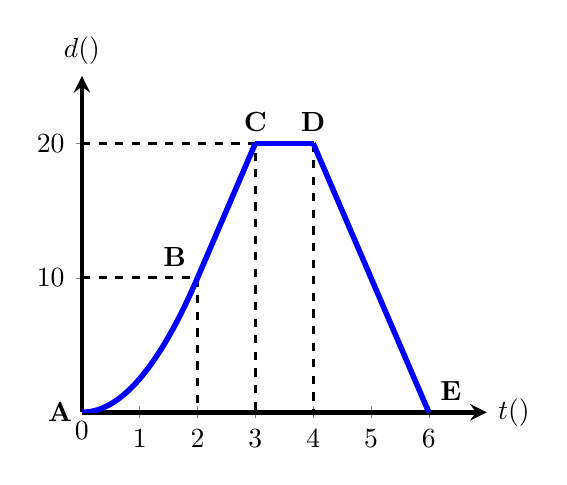
\begin{tikzpicture}  
			\begin{axis}[  ultra thick,scale=0.75,
				xmin=0,  
				xmax=7,  
				xtick={0,1,...,6},
				ytick={0,10,20},
				minor x tick num=0,
				minor y tick num=0,
				ymin=0,  
				ymax=25, 
				samples=300,
				axis lines=center, 
				xlabel=$\xsi{t}{\left(\si{\second}\right)}$, 		ylabel=$\xsi{d}{\left(\si{\meter}\right)}$,
				every axis y label/.style={at=(current axis.above origin),anchor=south},  
				every axis x label/.style={at=(current axis.right of origin),anchor=west},  ]
				\draw[dashed, line width=1pt] (axis cs: 0,10)--(axis cs: 2,10)--(axis cs: 2,0);
				\draw[dashed, line width=1pt] (axis cs: 0,20)--(axis cs: 3,20)--(axis cs: 3,0);
				\draw[dashed, line width=1pt] (axis cs: 4,20)--(axis cs: 4,0);
				\addplot [line width=2pt, blue, smooth, domain=0:2] {0.5*5*x^(2)}; 
				\addplot [line width=2pt, blue, smooth, domain=2:3] {10+10*(x-2)};  
				\addplot [line width=2pt, blue, smooth, domain=3:4] {20}; 
				\addplot [line width=2pt, blue, smooth, domain=4:6] {20-10*(x-4)};
				\coordinate (O) at (axis cs: 0,0);
				\coordinate (A) at (axis cs: 0,0);
				\coordinate (B) at (axis cs: 2,10);
				\coordinate (C) at (axis cs: 3,20);
				\coordinate (D) at (axis cs: 4,20);
				\coordinate (E) at (axis cs: 6,0);
				\node[above left] at (B) {\textbf{B}};
				\node[above] at (C) {\textbf{C}};
				\node[above] at (D) {\textbf{D}};
				\node[above right] at (E) {\textbf{E}};
			\end{axis}  
			\node[below] at (O) {0};
			\node[left] at (A) {\textbf{A}};
		\end{tikzpicture}
	\end{center}
	\choiceTF[t]
	{Trong khoảng thời gian từ $\SI{0}{\second}$ đến $\SI{6}{\second}$ thủ môn không đổi hướng chuyển động}
	{\True Thủ môn tăng tốc trong khoảng thời gian từ $\SI{0}{\second}$ đến $\SI{2}{\second}$}
	{\True Tốc độ chuyển động của thủ môn từ điểm B đến điểm C là $\SI{10}{\meter/\second}$}
	{\True Từ 4 giây đến 6 giây, vận tốc chuyển động của thủ môn có giá trị $\SI{-10}{\meter/\second}$}
	\loigiai{}
\end{ex}
% ===================================================================
\begin{ex}
Khi xe chạy trên đường cao tốc, xe phải giữ khoảng cách an toàn với xe phía trước để có thể xử lý kịp thời khi xe phía trước gặp sự cố.
\begin{center}
	\includegraphics[width=0.4\linewidth]{../figs/D10-1-4}
\end{center}	
Khoảng cách an toàn này tùy thuộc vào tốc độ xe và đã được nêu trong một số quy định của chính phủ. Tuy nhiên, để dễ nhớ, khi lưu thông vào ban ngày và khi đường khô ráo người ta thường tính toán theo một trong các quy tắc sau:
\begin{itemize}
	\item \textbf{\textit{Quy tắc 1:}} Quy tắc $\SI{3}{\second}$  tối thiểu. Khoảng cách an toàn tối thiểu bằng quãng đường xe đi được trong $\SI{3}{\second}$. Ví dụ xe chạy với tốc độ $\SI{72}{\kilo\meter/\hour}$  thì khoảng cách an toàn tối thiểu với xe phía trước là $\SI{60}{\meter}$.
	\item \textbf{\textit{Quy tắc 2:}} Quy tắc tương đương. Khoảng cách an toàn tối thiểu (theo đơn vị $\si{\meter}$) bằng tốc độ của xe (theo đơn vị $\si{\kilo\meter/\hour}$). Ví dụ tốc độ xe là $\SI{80}{\kilo\meter/\hour}$  thì khoảng cách an toàn tối thiểu với xe phía trước là $\SI{80}{\meter}$.
\end{itemize}
Một xe ô tô đang chạy trên đường cao tốc nằm ngang với tốc độ $\SI{108}{\kilo\meter/\hour}$  thì bất ngờ thấy một sự cố trên đường ở phía trước, sau đó $\SI{1}{\second}$ thì tài xế ô tô bắt đầu giảm hẳn ga và thắng gấp xe lại với gia tốc có độ lớn $\SI{8}{\meter/\second^2}$ cho đến khi xe ngừng lại.
	\choiceTF[t]
	{\True Theo quy tắc 1, khoảng cách an toàn tối thiểu với trường hợp xe ô tô trên là $\SI{90}{\meter}$}
	{Theo quy tắc 2, khoảng cách an toàn tối thiểu với trường hợp xe ô tô trên là $\SI{30}{\meter}$}
	{\True Tổng quãng đường ô tô đi được từ lúc phát hiện sự cố đến khi dừng lại $\SI{86.25}{\meter}$}
	{\True Nếu sự cố mà xe ô tô nhìn thấy là một xe container phía trước, đang chuyển động cùng chiều, thẳng đều, với tốc độ $\SI{36}{\kilo\meter/\hour}$ thì khoảng cách tối thiểu của hai xe kể từ lúc người lái ô tô thắng lại phải là $\SI{25}{\meter}$ để không xảy ra tai nạn. }
	\loigiai{
	\begin{itemchoice}
		\itemch Đúng.
		\itemch Sai. Theo quy tắc 2, khoảng cách an toàn tối thiểu là $\SI{108}{\meter}$.
		\itemch Đúng.\\
		Trong quá trình từ khi ô tô thấy sự cố đến khi thắng lại, ô tô chuyển động thẳng đều. Quãng đường ô tô đi được trong quá trình trên: $s_1=v_0t=30\cdot1=\SI{30}{\meter}$.\\
		Trong quá trình ô tô thắng lại, ô tô chuyển động chậm dần đều với vận tốc đầu $v_0$. Đến khi dừng lại  $v=0$.\\
		Quãng đường ô tô đi được trong quá trình này: $s_2=\dfrac{v^2-v^2_0}{2a}=\SI{56.25}{\meter}$.\\
		Tổng quãng đường ô tô đi được từ lúc phát hiện sự cố đến khi dừng lại: $s=s_1+s_2=\SI{86.25}{\meter}$.
		\itemch Đúng.\\
		Chọn trục tọa độ  gắn với xe con, chiều dương $Ox$ cùng chiều chuyển động của xe, gốc tọa độ O trùng với điểm B, gốc thời gian lúc ô tô bắt đầu hãm phanh.\\
		Phương trình chuyển động của ô tô: $x_1=-\mathrm{AB}+v_{01}t-\dfrac{1}{2}at^2$.\\
		Phương trình chuyển động của xe container:  $x_2=v_2t$.\\
		Nếu hai xe va chạm (gặp nhau): 
		$$x_1=x_1\Rightarrow \mathrm{AB}+\left(v_2-v_{01}\right)t+\dfrac{1}{2}at^2=0 \quad \left(*\right)$$
		Để ô tô chỉ gặp xe container một lần và dừng lại ngay trước khi va chạm, hoặc không gặp xe container (không xảy ra tai nạn) thì phương trình (*) phải có không quá một nghiệm thực, khi đó biệt số $\Delta $:
		$$\Delta \le 0\Leftrightarrow \left(v_2-v_{01}\right)^2-2a\cdot\mathrm{AB}\le 0$$
		$$\Rightarrow \mathrm{AB}\ge \dfrac{\left(v_2-v_{01}\right)^2}{2a}$$
		$$\Rightarrow \mathrm{AB}_{\text{min}}=\dfrac{\left(v_2-v_{01}\right)^2}{2a}=\SI{25}{\meter}.$$
	\end{itemchoice}
	}
\end{ex}
\Closesolutionfile{ans}

\section{Câu trắc nghiệm trả lời ngắn} \textit{Thí sinh trả lời từ câu 1 đến câu 6}
\setcounter{ex}{0}
\Opensolutionfile{ans}[ans/G10-4-TL]
	% ===============================================================
\begin{ex}
	Một nhóm học sinh đo được hiệu điện thế giữa hai đầu một điện trở là $U=\xsi{\left(10,0\pm0,3\right)}{\volt}$ và cường độ dòng điện qua điện trở là $I=\xsi{\left(1,3\pm0,2\right)}{\ampere}$. Tính sai số tương đối trong phép đo điện trở \textit{(Kết quả tính theo đơn vị $\si{\percent}$ và làm tròn đến 3 CSCN)}.\\
	Cho biết giá trị của điện trở được xác định bởi $R=\dfrac{U}{I}$.
	\shortans{18,4 }
	\loigiai{
		Giá trị điện trở:
		$$R=\dfrac{U}{I}.$$
		Sai số tương đối của phép đo:
		$$\delta R=\left(\dfrac{\Delta U}{\overline{U}}+\dfrac{\Delta I}{\overline{I}}\right)\cdot\SI{100}{\percent}\approx\SI{18.4}{\percent}.$$
	}
\end{ex}
% ===============================================================
\begin{ex}
	Một vận động viên chạy từ điểm xuất phát lên một quả đồi với tốc độ không đổi $\SI{3}{\meter/\second}$. Khi chạy được $\SI{90}{\meter}$ thì vận động viên này lập tức chạy ngược lại theo đường cũ về điểm xuất phát với tốc độ không đổi $\SI{6}{\meter/\second}$. Ở cả hành trình trên, tốc độ trung bình của vận động viên là bao nhiêu $\si{\meter/\second}$?
	\shortans{4 }
	\loigiai{
		$$v_{\text{tb}}=\dfrac{2s}{\dfrac{s}{v_1}+\dfrac{s}{v_2}}=\SI{4}{\meter/\second}.$$
	}
\end{ex}
% ===================================================================
\begin{ex}
	Một con bọ rùa bò đều trên các cạnh của một tấm ván hình chữ nhật với chiều dài các cạnh $\mathrm{AB}=\SI{40}{\centi\meter}$, $\mathrm{BC}=\SI{20}{\centi\meter}$, mỗi 2 giây nó bò được $\SI{1.5}{\centi\meter}$. Tại thời điểm ban đầu, con bọ rùa ở đỉnh A của tấm ván. Kể từ thời điểm ban đầu, trong thời gian $\SI{80}{\second}$, vận tốc trung bình là bao nhiêu $\si{\centi\meter/\second}$? \textit{(Kết quả làm tròn đến 2 chữ số sau dấu thập phân.)}
	\shortans{$0,56$}
	\loigiai{
	Trong $\SI{80}{\second}$ con bọ rùa bò được $\SI{60}{\centi\meter}$ nên đi được hết cạnh AC và BC.\\
	$$v=\dfrac{\sqrt{\mathrm{AC}^2+\mathrm{BC}^2}}{t}\approx\SI{0.56}{\centi\meter/\second}.$$
	}
\end{ex}
% ===============================================================
\begin{ex}
Một vật chuyển động thẳng có đồ thị vận tốc - thời gian như hình bên dưới. Tính tổng quãng đường vật đi được trong khoảng thời gian $\SI{12}{\second}$ theo đơn vị mét.
\begin{center}
	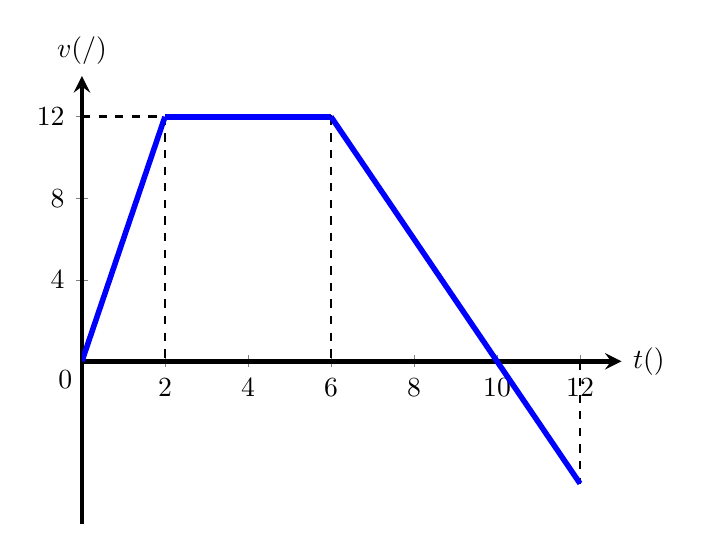
\begin{tikzpicture}  
		\begin{axis}[  ultra thick,
			xmin=0,  
			xmax=13,  
			xtick={0,2,...,12},
			ytick={0,4,...,12},
			ymin=-8,  
			ymax=14, 
			samples=300,
			axis lines=center, 
			xlabel=$\xsi{t}{\left(\si{\second}\right)}$, 		ylabel=$\xsi{v}{\left(\si{\meter/\second}\right)}$,
			every axis y label/.style={at=(current axis.above origin),anchor=south},  
			every axis x label/.style={at=(current axis.right of origin),anchor=west},  ]
			\draw[dashed, line width=1pt] (axis cs: 0,12)--(axis cs: 2,12)--(axis cs: 2,0);
			\draw[dashed, line width=1pt] (axis cs: 0,12)--(axis cs: 6,12)--(axis cs: 6,0);
			\draw[dashed, line width=1pt] (axis cs: 12,0)--(axis cs: 12,-6);
			\addplot [line width=2pt, blue, smooth, domain=0:2] {6*x}; 
			\addplot [line width=2pt, blue, smooth, domain=2:6] {12};  
			\addplot [line width=2pt, blue, smooth, domain=6:12] {12-3*(x-6)}; 
			\coordinate (O) at (axis cs: 0,0);
		\end{axis}  
		\node[below left] at (O) {0};
	\end{tikzpicture}
\end{center}	
	\shortans{$90$ }
	\loigiai{
		$$s=\dfrac{1}{2}\cdot\left(4+10\right)\cdot12+\dfrac{1}{2}\cdot2\cdot6=\SI{90}{\meter}.$$
	}
\end{ex}
% ===================================================================
\begin{ex}
	Một người đi xe đạp với tốc độ $v_1=\SI{5}{\meter/\second}$ bên cạnh đường ray tàu hỏa thì thấy một chiếc tàu hỏa chạy qua cùng chiều. Tốc độ của tàu hỏa là $v_2=\SI{15}{\meter/\second}$ đối với mặt đất. Sau thời gian $\SI{15}{\second}$ thì người đó thấy tàu hỏa vượt qua mặt mình. Chiều dài của tàu hỏa là bao nhiêu mét?
	\begin{center}
		\includegraphics[width=0.5\linewidth]{../figs/D10-1-2}
	\end{center}
\shortans{150}
	\loigiai{
		Vận tốc tương đối của tàu hỏa so với người:
		$$v_{21}=v_2-v_1=\SI{10}{\meter/\second}$$
		Chiều dài của tàu hỏa:
		$$L=v_{21}t=\SI{150}{\meter}.$$
	}
\end{ex}
% ===================================================================
\begin{ex}
	\immini{
		Trong khi làm thí nghiệm với đồng hồ đo thời gian hiện số, một học sinh chọn kiểu làm việc (MODE) của đồng hồ ở vị trí A và nối cổng quang điện với ổ A của đồng hồ. Học sinh này thả rơi một thước nhôm dài $\SI{20}{\centi\meter}$ theo phương thẳng đứng sao cho thước rơi qua cổng quang điện (thước luôn thẳng đứng khi rơi) thì thấy số chỉ của đồng hồ bằng $\SI{0.077}{\second}$. 
	}
	{\includegraphics[width=0.6\linewidth]{../figs/D10-1-1}}
	Bỏ qua sức cản của không khí và thước chuyển động nhanh dần đều với gia tốc có độ lớn $\SI{9.8}{\meter/\second^2}$. Khi thả, đầu dưới của thước cách cổng quang điện một khoảng bằng bao nhiêu? \textit{(Kết quả tính theo đơn vị centimet và làm tròn đến phần nguyên.)}
	\shortans{25}
	\loigiai{
		Gọi $v$ là vận tốc của thước khi đầu thước bắt đầu chắn qua cổng quang thì:
		$$\ell=vt+\dfrac{1}{2}at^2\Leftrightarrow 0,2=v\cdot0,072+\dfrac{1}{2}\cdot9,8\cdot0,072^2\Rightarrow v\approx\SI{2.22}{\meter/\second}.$$
		Khoảng cách từ đầu thước đến cổng quang lúc thả:
		$$h=\dfrac{v^2}{2a}\approx\SI{0.25}{\meter}=\SI{25}{\centi\meter}.$$
	}
\end{ex}

\Closesolutionfile{ans}
\begin{center}
	\textbf{-- HẾT --}
\end{center}